\section{Experimental analysis}

We implemented various algorithms presented in this paper, and experimentally compare their performance for string similarity joins with taxonomies. The experiments study both the effectiveness and efficiency of proposed measures and join algorithms.  


 

\subsection{Experimental setting and datasets}

We  implemented all similarity measurement and algorithms in Java $1.6.0$ and run on a
Windows XP with dual-core Intel Xeon CPU 4.0GHz, 2GB RAM, and a 320GB hard disk.


We use three real datasets and one random dataset: Consensus data (\textbf{Consensus}),
Crimes data  (\textbf{Crime}), and Life science data
(\textbf{Life}) and three taxonomies. These datasets differ from each other in terms of data-size and string-length, taxonomy-size, taxonomy-tree-complexity, . Our goal in choosing these diverse sources is to understand the usefulness of algorithms in different real world environments.


\smallskip
%\noindent \textbf{{Consensus data}}: Extraction was done by Barry Becker from the 1994 Census database. native-country: Include 32561 instances, we can perform the similarity joins on multiple column, including countries, occupation, marital-status, education and workclass. The feature of this dataset is to perform the similarity join against multiple columns.

\noindent \textbf{{Crime data}}: This dataset reflects reported incidents of crime that occurred in the City of Chicago from 2001 to present \footnote{https://catalog.data.gov/dataset/crimes-2001-to-present-398a4}. The dataset contains more than 65,000 records/rows of data and cannot be viewed in full in Microsoft Excel.


\noindent \textbf{{Library data}}: This dataset\footnote{http://www.theeuropeanlibrary.org/tel4/access/data/opendata/details}  constitutes the subset of The European Library's aggregated data that is made openly available by its partner libraries. 




\noindent \textbf{{Life science data}}: As a subject matter taxonomy for our expert matching
in this medicine domain, we used the Medical Subject Head-
ings (MeSH)\footnote{https://www.nlm.nih.gov/mesh} that is a biomedical controlled vocabulary
consisting of 26k+ biomedical terms arranged in a taxonomic
structure introduced by National Library of Medicine
(NLM). The benefits of using MeSH terms have been increasingly
highlighted in various applications for biomedical
concept and knowledge extraction from text [11]. We obtained one million gene/protein records
from the Expasy website ({\footnotesize http://www.expasy.ch/sprot}).
Each record contains an identifier (ID) and its name. In this dataset, each ID has $5\sim22$ synonyms. We generated 10,000 synonym rules describing gene/protein
equivalent expressions.

\noindent \textbf{{Synthetic data}}: We generate data by random creating a taxonomy tree with varied tree fanout and tree depth. 

\begin{table}[t]
\centering
\begin{tabular}{|@{\hspace{1mm}}c@{\hspace{1mm}}|@{\hspace{1mm}}c@{\hspace{1mm}}|@{\hspace{1mm}}c@{\hspace{1mm}}|@{\hspace{1mm}}c@{\hspace{1mm}}|}
%{|p{1cm}|p{1cm}|p{1cm}|p{1cm}|p{1cm}|p{1cm}|p{1cm}|}
%|c|m{6cm}|
\hline
 \textbf{Name} & \textbf{\# of nodes} &  \textbf{Depth} & \textbf{Fan-out} \\
  \hline \hline

  Wikipedia & 10,000 & 5 & 2,000 \\

   MeSH category  & 56326 & 5 &  18/3.4 \\

  WordNet & 10,000  & 5 & 2,000  \\

  \hline
\end{tabular}
\caption{Characteristics of taxonomy datasets.}
\label{tab:data}
\end{table}

\begin{table}[t]
	\centering
	\begin{tabular}{|@{\hspace{1mm}}c@{\hspace{1mm}}|@{\hspace{1mm}}c@{\hspace{1mm}}|@{\hspace{1mm}}c@{\hspace{1mm}}|@{\hspace{1mm}}c@{\hspace{1mm}}|}
		%{|p{1cm}|p{1cm}|p{1cm}|p{1cm}|p{1cm}|p{1cm}|p{1cm}|}
		%|c|m{6cm}|
		\hline
		\textbf{Name} & \textbf{\# of records} &  \textbf{Length} & \textbf{\# of T-node per string} \\
		\hline \hline
		
		Crime records & 10,000 & 5 & 2,000 \\
		
		MeSH terms  & 935249 & 2.1 &  1.5/9 \\
		
	    Library records & 36,000  & 5 & 2,000  \\
		
		\hline
	\end{tabular}
	\caption{Characteristics of join datasets.}
	\label{tab:data}
\end{table}


%\begin{figure}
%  \small
%  \centering
%  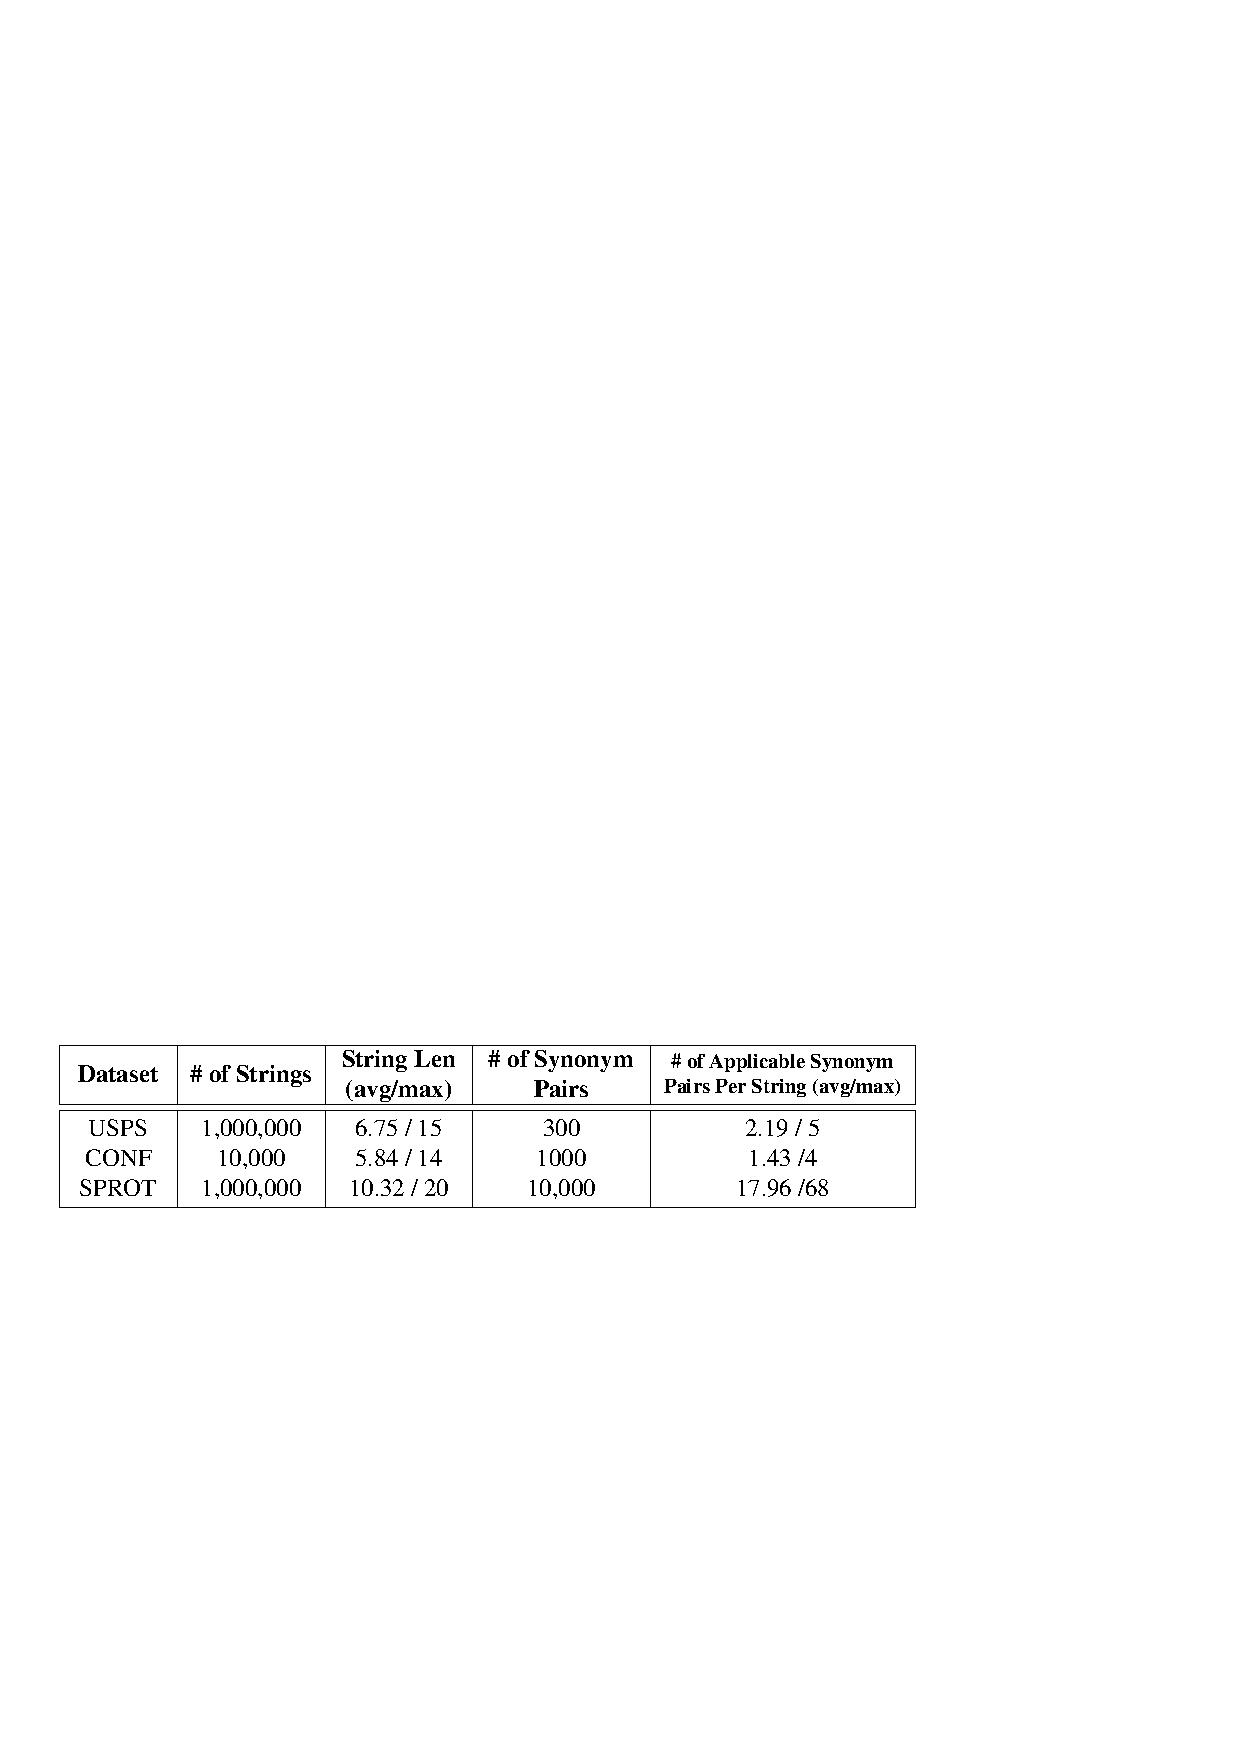
\includegraphics[width=\linewidth]{figures/Characteristics_Datasets}
%   \vspace{-6mm}
%  \caption{Characteristics of Datasets.}
%  \label{tab:data_characteristics}
%\end{figure}


Figure~\ref{tab:data_characteristics} gives the characteristics of the
three datasets.

\subsection{Effectiveness of taxonomy for string joins}

The first experiment is to demonstrate the effectiveness of
taxonomy for string joins. We compared our
two measures: Jaccard similarity, full expansion
  (\textbf{Full}), and  our similarity with taxonomy.

For each of the three datasets, we performed the experiments by conducting a similarity join between the
query table $T_Q$ and the target table $T_T$ as follows: (1) $T_Q$ consists of 100 manually selected
full names, and (2) $T_T$ has 500 records where 100 of them
are the correct abbreviations of the corresponding records in $T_Q$
(i.e., the ground truth), and the other 400 random records are selected from string collections. This is to
ensure that there is only one correct matching record in $T_T$ for each
 record in $T_Q$.

Quality of Measures.

In Figure \ref{fig:quality}, we report the quality of the measures by testing the \textit{Precision} (short for ``P''),  \textit{Recall} (``R''), and \textit{F-measure$=\frac{2\times P \times R}{P+R}$} (``F'') on three datasets. We observe that:

\noindent$\bullet$ The similarity measures using synonyms (including \textit{JaccT}, \textit{Full} and \textit{SE}) obtain higher scores than Jaccard which does not consider synonym pairs. The reason is that without using synonyms, Jaccard has no chance to improve the similarity.

%\noindent$\bullet$  \textit{Full} achieves a comparable performance with \textit{JaccT}. Note that \textit{JaccT}  selects only appropriate synonyms to increase the similarity, but \textit{Full} utilizes all the applicable rules and most rules in \textit{Full} is useful, since it is not common that synonyms contain ambiguous meanings. In addition, note hat \textit{Full} is much more efficient than \textit{JaccT}, which will be demonstrated later.


\noindent$\bullet$ \textit{SE} significantly outperforms \textit{JaccT} in each dataset. For example, on SPROT dataset, the F-measures of \textit{SE} and \textit{JaccT} are $0.82$ and $0.52$, respectively. The main reason is that: an abbreviation may have various full expressions and the join records may contain the combination of multiple expressions. Therefore \textit{SE} can apply multiple rules, while \textit{JaccT} can apply only one. Note that such situation is not rare in the real world, as one fragment of a string likely involves multiple synonym rules. We illustrate one example on each of three datasets in Figure \ref{fig:quality} to compare the performance of four similarity measures. For example, see CONF data in Figure \ref{fig:quality}, ``\textsf{VLDB}'' has two different full expressions, i.e., ``\textsf{International Conference on Very Large Databases}'' ($r_1$) and ``\textsf{Proceedings of the VLDB Endowment}''($r_2$), and $s1$ contains these two expressions.  \textit{SE} applies both $r_1$ and $r_2$ to $s_2$ to obtain a high similarity score, i.e., 0.93, while \textit{JaccT} can only apply $r_2$ to $s_2$ and the similarity is only $0.57$. Assume that the join threshold is 0.8, then  \textit{JaccT} can not find the correct answer while \textit{SE} can.


\begin{figure*}[h]
	\small
	\centering
	\includegraphics[width=\linewidth]{figures/measure01}
	\caption{Quality of similarity measures (P: precision, R: recall, F: F-measure) and examples to illustrate the quality of similarity measures. }
	\label{fig:quality}
\end{figure*}

\begin{figure}[t]
	\centering
	\includegraphics[scale=0.25]{figures/TrieJoin}
	\caption{Three join algorithms}
	\label{fig:similaritygeaph}
\end{figure}

\begin{figure}
	\centering
	\includegraphics[scale=0.25]{figures/LCPTimes}
	\caption{LCP times for two algorithms}
	\label{fig:LCPTimes}
\end{figure}

\begin{figure}
	\centering
	\includegraphics[scale=0.25]{figures/selectratio}
	\caption{Three algorithms with varied selectivity ratios (5M records, random data)}
	\label{fig:selectratio}
\end{figure}

\subsection{Efficiency and scalability of exact-join algorithms}

The second set of experiments is to test the efficiency and scalability of
various exact-joins algorithms. We compared our algorithms, the \textbf{baseline}
and \textbf{TIndex}.

Metrics.

 We took the following measures: (i) the running time (including filtering time, verification time and the time for building QP-tree for a query), and (ii) the size of candidates.

Running Time and Scalability.
Figure~\ref{fig:search_scalability_datasize} shows the running time of the four search algorithms, where the threshold is $0.9$. As shown, the running times of Search-baseline(F) and Search-baseline(S) have an exponential growth, whereas QP-search(F) and QP-search(S) scale better (i.e., linear). The reason is that QP-search generates less candidates for the final verification.

To study the scalability of algorithms with the various threshold values, we plotted Figure \ref{fig:search_scalability_threshold}. As shown, the running time of the algorithms decreases with the growth of the threshold values. In addition,  QP-search scales well with various thresholds. In contrast, when the threshold value is small, the running time of Search-baseline increases significantly. For example, in Figure \ref{fig:search_scalability_threshold}(b), when threshold=0.9, the running time of Search-baseline is about 7 times more than that of QP-search. In addition, when the threshold=0.5, the performance of QP-search is at least 15 times better than Search-baseline.

We then study the time cost of Search-baseline and QP-search with different number of synonyms. Recall that the similarity search proceeds to  generate signatures (or QP-index) for a given query, and then to filter the candidates by checking the overlaps of the signatures, and finally to verify the similarity. Therefore, we reported the individual execution time of signature-generation, filtering and verification in Figure  \ref{fig:search_synonyms_conf}. As seen from this figure, we observe that QP-Search(S) significantly outperforms Search-baseline(S) by one order of magnitude. The main reasons are as follows:



(i)  Search-baseline(S) needs to union all the signatures computed from each possible expanded set, while QP-Search(S) directly utilizes the intermediate signatures. Therefore, the time of signature-generation of QP-Search(S) is less than that of Search-baseline(S).

(ii) For the filtering phase, QP-Search(S) utilizes the SI-Index and QP-index to achieve stronger filtering power than Search-baseline(S). Thus, the filtering time of QP-Search(S) is less than Search-baseline(S). In addition, due to the powerful filtering, QP-Search(S) generates less candidates than that of Search-baseline(S). For example, in Figure  \ref{fig:search_synonyms_conf}, we reported the number of candidates for each query. As shown, the number of candidates of Search-baseline(S) is about one order of magnitude more than that of QP-search(S).

(iii)  QP-Search(S) spends less time on verifying the candidates than Search-baseline(S). Therefore, the verification time of QP-Search(S) is less than that of Search-baseline(S).

Therefore, QP-Search(S) outperforms Search-baseline(S) in each of the three phases.  Experiments in USPS and SPROT datasets have the similar trend (as shown in Figure \ref{fig:search_synonyms_usps} and Figure \ref{fig:search_synonyms_sprot}, respectively).

\subsection{Efficiency and scalability of approximate-join algorithms}

The third set of experiments is to test the efficiency and scalability of
approximate-join algorithms. We compared the algorithms \textbf{baseline}
and \textbf{SI-Join}.  We implemented all algorithms using both
prefix and LSH filters. Therefore, with respect to the algorithms using
LSH scheme, we append ``-LSH'' to the name, e.g., JaccT-LSH denotes the
JaccT algorithm using LSH scheme. Note that, we use the false negative
ratio $\delta \leq 5\%$, i.e., the accuracy is $1-\delta \geq 95\%$. The
parameters $k$ and $l$ should satisfy: $\delta \geq
(1-\theta^k)^l$~\cite{journals/tods/XiaoWLYW11}. For example, if
threshold $\theta=0.8$, $k=3$, then $l$ should be at least $5$ to
guarantee $> 95\%$ accuracy.

Metrics. We took the following measures: (i) the size of signatures, (ii) the filtering ratio of the algorithms, which is typically defined as the number~of~pruned~string~pairs divided by the total number of string pairs; and (iii) the running time (including filtering time and verification time).

Number of Signatures.


We first performed experiments to report the number of signatures of a
query string. It has a major impact on the query time, as both \textit{JaccT} and
our join algorithms need to frequently check the overlaps of string
signatures. The results are reported in Figure~\ref{fig:signature-size}.
For both prefix and LSH schemes, the number of signatures of our
expansion-based algorithms is smaller than that of \textit{JaccT}. The reason is
that based on a transformation framework, \textit{JaccT} is more likely to
include new tokens into signatures than ours. In addition, we observe
that the size of signatures in the LSH scheme is greater than that in
prefix scheme, and the gap increases when the threshold decreases. As we
will see shortly, this results in substantial overhead of filtering time
for the LSH scheme.


\textbf{Filtering Power.}

We investigated the filtering power of different algorithms in
Figures~\ref{fig:filter_ratio_prefix} and \ref{fig:filter_ratio_LSH} using
prefix and LSH schemes, respectively. The experiments were performed on
USPS and SPROT datasets for self-join. For prefix-based algorithms,
Join-baseline is slightly better than JaccT, while SI-Join has a substantial
lead over JaccT and Join-baseline. These results are mainly because of the
additional filtering power in SI-Join brought by length filtering and
signature filtering. Next, for LSH-based algorithms, Figure
\ref{fig:filter_ratio_LSH} demonstrates the similar trend. That is,
SI-Join is the winner in all settings by varying the parameters $k$ and
$l$. Compared to the prefix scheme, LSH has a slightly higher filtering
ratio when parameters are set optimally (e.g. 99.2\% v.s. 98.9\% in USPS
data, with threshold 0.9). On the other hand, note that LSH may filter
away correct answers, resulting in false negatives, as can be seen from
the false negative percentages shown in
Figure~\ref{fig:filter_ratio_LSH}.

\textbf{Effects of different filters.}

We analyzed the effects of different filters, i.e., signature-filters, length-filters and  signature-plus-length. As shown in Figure \ref{fig:filter_methods},  signature-plus-length filters obtain the strongest filtering power on all the datasets, which explains why our algorithms use these two kinds of filters together. There is no absolute winner between signature filters and length filters. In particular, signature filters have stronger filtering power on the USPS dataset (Figure \ref{fig:filter_methods}(a)), while the opposite situation occurs in the SPROT dataset (Figure \ref{fig:filter_methods}(c)), i.e., length filters beat signature filters. On the CONF dataset (Figure \ref{fig:filter_methods}(b)), when the threshold value is small, signature filters win length filters. However, when the threshold value is high, length filters beat signature filters. Therefore, the individual effects of signature filters and length filters depend on the data sets and the thresholds, and the combined structure of both (i.e. SI-tree) achieves the best results.



\begin{figure}[t]
	\centering
	\includegraphics[scale=0.25]{figures/Drawing1}
	\caption{Nested loop and SS filter}
	\label{fig:similaritygeaph}
\end{figure}


\textbf{Running Time and Scalability.}


Figure~\ref{fig:scalability} and Figure \ref{fig:scalability_LSH} show the running time of five join algorithms based on prefix and LSH schemes, respectively, where the join threshold is $0.8$. The x-axis represents the join data size. As shown, the running times of both JaccT and Join-baseline (i.e., Join-baseline(F), Join-baseline(S)) have an exponential growth, whereas SI-Join (i.e., SI-Join(F), SI-Join(S))  scales better (i.e., linear) than Join-baseline and JaccT. The reason is that SI-Join methods have more efficient filtering strategies and generate smaller size of candidates.  In addition, in order to study the scalability of algorithms with the increase of the number of rules, we plot Figure \ref{fig:synonyms}(b), where  SI-Join(F) (i.e., SI-Join with the full-expansion) is a clear winner in algorithms using rules: it is insensitive to the number of rules and thus able
to outperform other methods when one string involves more than 10 rules.


\smallskip

\subsection{Estimation-based filter selection}

The following tables shows the results for our estimation and the optimal filters by trying all possibilities. This is the join operations for all 1K data self-joins.

By varying the thresholds:

Thresholds: 0.75, Optimal 19.25K candidate, estimation: 19.30K

Thresholds: 0.8, Optimal 19.8K candidate, estimation: 19.9K

Thresholds: 0.85, Optimal 20.1K candidate, estimation: 20.8K

Thresholds: 0.9, Optimal 16.7K candidate, estimation: 18.4K

Thresholds: 0.95, Optimal 18.8K candidate, estimation: 19.05K

\noindent \textbf{Summary} ~~ Finally, we summarize the main findings.

(1) Considering four similarity measures, we observe that \textit{Jaccard} is inadequate due to its complete neglect of synonym rules. \textit{JaccT} is not efficient because it enumerates all transformed strings and entails large query overhead. \textit{Full-expansion} is extremely efficient, but its F-measure is not as good as \textit{Selective-expansion}, which makes a good balance between effectiveness and efficiency.

(2)	With respect to the similarity searches and joins,  QP-search and SI-join are the winners in the settings, respectively over the previous algorithms (i.e., \textit{JaccT}) and baseline methods. Note that we achieve a speedup of up to 50$\sim$300x on three data sets over the state-of-the-art approach.

(3) Finally, 2DHS synopsis offers very good results, and is extremely efficient to estimate the filtering power of different filters, ( $<$ 1 second ,  accounting for only 1\% of the total running time),  which strongly motivates its application in practice.

